\clearpage
\hypertarget{conBran vis}{}
\subsection{Visual; (original appendix text)}
\visHeader

\begin{itemize}
  

\item[$\blacktriangleright$] Edit the \texttt{Box} class in your metamodel by invoking the \texttt{Operations} dialogue and create a new method called
\texttt{initalizeBox}. Recalling the sole condition of this feature, set its return type as \texttt{EBoolean}. Save the method, then open the \texttt{grow} SDM.

\item[$\blacktriangleright$] Add a new \texttt{StatementNode} named \texttt{initialize}. In the \texttt{Statement} tab, invoke a \texttt{MethodCallExpression},
using the \texttt{this} object to access your new method.

\item[$\blacktriangleright$] Attach two \texttt{StopNode}s to this statement, one \texttt{true} upon \texttt{success}, and one \texttt{false} upon
\texttt{failure}. The new additions should resemble Fig.~\ref{fig:newGrowControl}.

\begin{figure}[htp]
\begin{center}
  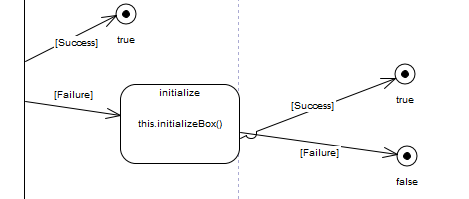
\includegraphics[width=0.7\textwidth]{ea_growControlAddition}
  \caption{caption}
  \label{fig:newGrowControl}
\end{center}
\end{figure}


\item[$\blacktriangleright$] Given that we now have our desired control flow, save, validate, and build your metamodel in Eclipse. Open \texttt{BoxImpl.java},
and go to the \texttt{grow} declaration, starting at (approximately) line 207. Scan the comments until you find \texttt{``//satement node initialize''}.

\begin{figure}[htp]
\begin{center}
  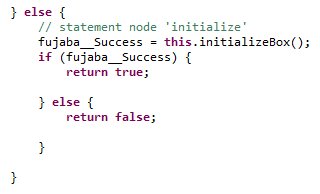
\includegraphics[width=0.5\textwidth]{eclipse_boxImplStatementNode}
  \caption{caption}
  \label{fig:initBoxImpl}
\end{center}
\end{figure}

\item[$\blacktriangleright$] Remember - the purpose of SDMs is to model \emph{control flow} -- this is \emph{not} where you'll define the function! Instead,
press \texttt{ctrl} and click on \texttt{initializeBox()}. This will automatically take you to its declaration (Fig.~\ref{fig:initBoxDecl}).

\begin{figure}[htp]
\begin{center}
  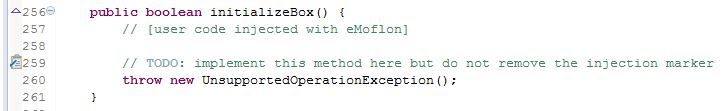
\includegraphics[width=\textwidth]{eclipse_initializeBoxDeclaration}
  \caption{caption}
  \label{fig:initBoxDecl}
\end{center}
\end{figure}

\item[$\blacktriangleright$] Before writing the needed Java code, lets review the goal of this pattern. We want to create two new boxes if and only if there are
\emph{no} partitions (i.e., no partition structure exists). This means we'll need to create a NAC!
 
 \fancyfoot[R]{ $\triangleright$ \hyperlink{return conBran}{Next}}

\end{itemize}
